
%% ------------- English version ---------------
\documentclass[english]{sbrt}
\usepackage[english]{babel}
\usepackage[utf8]{inputenc}
\usepackage[acronym]{glossaries}

\newtheorem{theorem}{Theorem}

\usepackage{booktabs}
\usepackage{multirow}
\usepackage{array}
\usepackage{graphicx}
\usepackage{subcaption}
\usepackage{amsfonts}
\usepackage{xcolor}
\usepackage{tikz}
%% ---------------------------------------------

\begin{document}

\newacronym{sbrt}{SBrT}{Brazilian Telecommunication Society}
\newacronym{sbrt2026}{SBrT~2026}{XLIV Brazilian Symposium on Telecommunication and Signal Processing}
\newacronym{ufba}{UFBA}{Federal University of Bahia}

\newacronym{ibge}{IBGE}{Brazilian Institute of Geography and Statistics}
\newacronym{anatel}{ANATEL}{Brazilian National Telecommunications Agency}
\newacronym{iqs}{IQS}{Service Quality Index}
\newacronym{rqual}{RQUAL}{Regulation on the Quality of Telecommunications Services}
\newacronym{dvr}{DVR}{Reference Values Document}
\newacronym{qos}{QoS}{Quality of Service}
\newacronym{qoe}{QoE}{Quality of Experience}
\newacronym{knn}{$k$NN}{$k$-Nearest Neighbors}
\newacronym{gnn}{GNN}{Graph Neural Networks}
\newacronym{pca}{PCA}{Principal Component Analysis}

\newcommand{\iqsrev}{\mathrm{IQS}_\mathrm{rev}}
\newcommand{\iqsleg}{\mathrm{IQS}_\mathrm{leg}}

\newcommand{\Xraw}{\mathbf{X}^\mathrm{raw}}
\newcommand{\xraw}{\mathbf{x}^\mathrm{raw}}

\newcommand{\Xpareto}{\mathbf{X}^\mathrm{pareto}}
\newcommand{\xpareto}{\mathbf{x}^\mathrm{pareto}}

\newcommand{\Xmodel}{\mathbf{X}^\mathrm{model}}
\newcommand{\xmodel}{\mathbf{x}^\mathrm{model}}

\newcommand{\Xlog}{\mathbf{X}^\mathrm{log}}
\newcommand{\xlog}{\mathbf{x}^\mathrm{log}}

\title{Manifold Ranker: A GNN-Based Framework for\\Multi-Objective Telecommunications Quality Ranking}

\author{Gabriel Luiz Espindola Pedro, Paulo Ricardo Branco da Silva, Arthur Cadore Matuella Barcella,\\ João Vitor Rosa Negri, Dimas Irion Alves, \textcolor{red}{and Anatel authors}
\thanks{Gabriel Luiz Espindola Pedro, Paulo Ricardo Branco da Silva, Arthur Cadore Matuella Barcella, João Vitor Rosa Negri, and Dimas Irion Alves are with Telecommunications Department of Aeronautics Institute of Technology, São José dos Campos, SP, Brazil, e-mails: \{gabrielluizep, arthurcadore, negri, pbranco, dimasirion\}@ita.br; \textcolor{red}{Anatel authors are with Anatel e-mails: \{xxx, yyy\}@anatel.gov.br}. This study was financed in part by the Coordenação de Aperfeiçoamento de Pessoal de Nível Superior - Brasil (CAPES) - Finance Code  001, Anatel under Decentralized Execution Agreement (TED) No. 03/2023, Work Program: 24.722.2205.20ZD.0001, and São Paulo Research Foundation (FAPESP) under grant 2020/09838-0 (BIOS---Brazilian Institute of Data Science).}%
}

\maketitle

\markboth{XLIV BRAZILIAN SYMPOSIUM ON TELECOMMUNICATIONS AND SIGNAL PROCESSING - SBrT 2026, SEPTEMBER 29--OCTOBER 02, 2026, SALVADOR, BA}{}


\begin{abstract}
Assessing the quality of telecommunications services across municipalities with heterogeneous structural, geographic, and socioeconomic conditions requires methodologies that go beyond simple weighted averages. This paper introduces Manifold Ranker, a \gls{gnn}-based self-supervised ranking framework that learns the geometry of municipality-level telecom quality indicators on a $k$-nearest-neighbor graph and produces a unified ranking score. The proposed architecture employs Residual Graph Convolutional layers and is trained with a multi-objective loss function that simultaneously enforces pairwise ranking consistency, input reconstruction fidelity, geometric smoothness on the learned manifold, and directional alignment with a Pareto-inspired proxy. We validate the approach on a longitudinal dataset covering Brazilian municipalities over multiple monthly periods, totaling over 82{,}000 municipality--period observations. Results show that the proposed model produces scores with a substantially wider effective range (standard deviation of 0.098) compared to the legacy \gls{iqs} (0.054) and revised \gls{iqs} (0.058) baselines, improving rank discrimination. Distribution and geographic visualizations confirm that the framework yields well-distributed and distinguishable municipality rankings, overcoming the saturation that affects current regulatory composites.
\end{abstract}

\begin{keywords}
Learn to Rank, Graph Neural Networks, Manifold Learning, Multi-Objective Optimization, Quality of Service
\end{keywords}


\section{Introduction}

Ranking municipalities in terms of telecommunications \gls{qos} poses a fundamental challenge to regulatory agencies. Such rankings are valuable not only for diagnostic purposes but also for technical and economical evaluation of specific municipalities or regions.

Defining a suitable ranking strategy is not trivial. The multi-dimensional nature of telecommunication performance---spanning voice, data, latency, coverage, and user satisfaction---means that different indicators can lead to conflicting orderings, a classical characteristic of multi-objective optimization problems. Furthermore, no established ground-truth ranking exists; evaluating model outputs depends on contextual domain knowledge rather than objective comparison. Selecting the essential variables is equally unclear: not only \gls{qos} indicators are required, but also covariates such as infrastructure and \gls{qoe} indicators.

Currently, regulatory agencies address this problem through linear composites. \gls{anatel} defined the \gls{iqs} through the \gls{dvr}, which encapsulates \gls{qos} metrics into a single-valued score for each municipality--period pair. However, this pointwise approach lacks a global overview of the municipalities' relative performance. By not considering pairwise dominance relationships between entities, the resulting scores become indistinguishable: similar entities are attributed near-identical values, and occurrences are clustered on narrow regions of the support domain. As our analysis shows, the legacy \gls{iqs} concentrates $50\%$ of all observations between $0.835$ and $0.863$, an interquartile range of merely $0.028$.

In multi-objective settings, Pareto dominance provides a natural partial ordering: municipality $A$ dominates municipality $B$ if $A$ is at least as good in every dimension and strictly better in at least one. However, many municipality pairs are incomparable under strict Pareto ordering, motivating the use of learned scalarizations that can resolve these ambiguities while still respecting the geometric structure of the data.

To address all the presented challenges, we propose Manifold Ranker, a \gls{gnn}-based Pareto-inspired model that learns the geometry of the feature space through a constructed \gls{knn} graph and, by entity pairwise competition, regresses a score value $s_i$ for each municipality $i$. This multi-objective optimization scheme contributes to an improved optimization landscape compared to unidimensional scalar optimizations, expanding the effective range of the target variable and thus enhancing discriminability.

The remainder of the paper is organized as follows.
Section~\ref{sec:dataset} presents the data used in this work and the currently calculated scores.
Section~\ref{sec:methodology} explains the concepts and presents the developed Manifold Ranker model.
Section~\ref{sec:results} presents the achieved results and a comparison with the currently applied strategies.
Section~\ref{sec:conclusions} concludes with final remarks.


\section{Dataset and Baseline Creation} \label{sec:dataset}

For the dataset construction we acquired \gls{qos} and \gls{qoe} indicators, and infrastructure covariates provided by \gls{anatel},
creating a matrix $\Xraw \in \mathbb{R}^{N \times D}$, where $N$ corresponds to the number of municipality--period entities and $D$ corresponds to the number of features.
$\Xraw$ is indexed by two keys: \textit{month}, which identifies the observation period, 
and \textit{municipality}, the official \gls{ibge} numeric code that uniquely identifies each municipality. 
Each row therefore corresponds to one municipality--month pair.

As \gls{qos} features we selected eight indicators normalized to $[0,1]$ with higher values denoting superior performance:
$\mathrm{IND}_1$ (voice-call connection rate), 
$\mathrm{IND}_2$ (voice-call drop rate, complemented),
$\mathrm{IND}_3$ (data-connection rate),
$\mathrm{IND}_4$ (download and upload speed compliance rate),
$\mathrm{IND}_5$ (data-connection latency, complemented),
$\mathrm{IND}_6$ (jitter, complemented),
$\mathrm{IND}_7$ (packet-loss rate, complemented), and
$\mathrm{IND}_8$ (service availability rate). 
For \gls{qoe}, the $\mathrm{ISG}$ (General Satisfaction Index) was selected as a composite of \gls{qoe} indicators for a given municipality--period tuple.
Infrastructure is represented by the $\mathrm{IBC}$ (Brazilian Coverage Index)
and the $\mathrm{INF4}_{\mathrm{UP},\{\mathrm{3G,4G,5G}\}}$ and $\mathrm{INF4}_{\mathrm{DL},\{\mathrm{3G,4G,5G}\}}$ indicators, which record the median upload and download speeds over each mobile data technology.

To establish a baseline comparison with regulatory approaches, we present the legacy \gls{iqs} and the recently revised \gls{iqs}, both of which linearly combine the same \gls{qos} features used in the model.

\subsection{Legacy IQS}

The legacy composite, $\iqsleg$, aggregates the $K$ normalized
technical \gls{qos} indicators through a fixed regulator-defined convex
combination,
\begin{equation}
    \iqsleg = \sum_{k=1}^{K} w_k^{\mathrm{leg}} \, \mathrm{IND}_k,
    \label{eq:qos_leg}
\end{equation}
each $\mathrm{IND}_k \in [0,1]$ is a normalized technical indicator, and the weight vector $w^{\mathrm{leg}} \in \Delta^{K-1}$
lies on the probability simplex. Under the legacy specification, the weights are fixed at
$w^{\mathrm{leg}} = (0.1,\, 0.1,\, 0.1,\, 0.2,\, 0.1,\, 0.1,\, 0.1,\, 0.2)$,
assigning greater relevance to $\mathrm{IND}_4$ and $\mathrm{IND}_8$.


\subsection{Revised IQS}

The revised composite, $\iqsrev$, replaces the fixed weights
with a performance-dependent scheme combined with a coverage bonus. The indicators are
first ranked from worst to best within each municipality, and the
weight assigned to rank position $r$ is
\begin{equation}
    \alpha_r = \frac{1}{r \, H_K},
    \label{eq:alpha_r}
\end{equation}
where $H_K = \sum_{j=1}^{K} 1/j$ is the $K$-th harmonic number. The revised composite
is then
\begin{equation}
    \iqsrev = \sum_{r=1}^{K} \alpha_r \cdot \mathrm{IND}_{\pi(r)} + B_{\mathrm{cov}},
    \label{eq:qos_rev}
\end{equation}
where $\pi$ is the permutation ordering indicators from worst to best performance, and
$B_{\mathrm{cov}}$ is a coverage bonus of five points
added whenever 4G or higher technology coverage in the urban area
reaches at least 95\%. The
inverse-harmonic weighting assigns greater importance to the worst-performing indicators,
penalizing municipalities with critical technical deficiencies.

\section{Methodology} \label{sec:methodology}

The proposed Manifold Ranker framework consists of a pipeline that transforms raw municipality indicators into a scalar ranking score through graph-based learning. Fig.~\ref{fig:pipeline} presents an overview of the process, which is detailed as follows.

\begin{figure*}
    \centering
    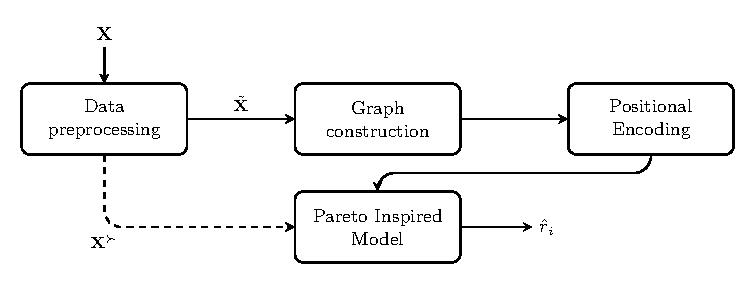
\includegraphics[width=1\linewidth]{figures/pipeline.pdf}
    \caption{Pipeline for the proposed methodology. Raw features $\Xraw$ are preprocessed into $\Xmodel$ (for graph construction and model input) and $\Xpareto$ (as a training proxy). A \gls{knn} graph is built, positional encodings are computed, and the \gls{gnn} model produces the final score $\mathbf{s}$.}
    \label{fig:pipeline}
\end{figure*}

\subsection{Preprocessing}

The selected data is composed of heavy-tailed, heterogeneous distributions common among infrastructure indicators. To transform the data into a suitable representation for neural optimization, we define a multi-stage preprocessing pipeline.

To reduce the dynamic range of features that follow power-law or log-normal-like distributions, we apply a Log1p transformation:
\begin{equation}
    \Xlog = \log(1+\Xraw).
    \label{eq:log1p}
\end{equation}

\noindent
This transformation prevents the undefined $\log(0)$ by the additive unit while compressing large values sublinearly.

To mitigate the effect of outliers, we apply a Robust Scaler that standardizes using robust statistics within the interquantile range $\{0.05, 0.95\}$:
\begin{equation}
    \tilde{x}_{i,j} =
        \frac{\xlog_{i,j} - \mathrm{median}(\xlog_{:,j})}
        {Q_{0.95}(\xlog_{:,j})-Q_{0.05}(\xlog_{:,j})}.
    \label{eq:robust_scaling}
\end{equation}

From the robust-scaled features, we apply Standard Scaling to center variables to zero mean and unit variance, improving conditioning for first-order optimizers:
\begin{equation}
    \Xmodel_{i,j} = \frac{\tilde{x}_{i,j} - \mu_j}{\sigma_j},
    \label{eq:std_scaling}
\end{equation}

\noindent
where $\mu_j$ and $\sigma_j$ are the mean and standard deviation for feature $j$ across all entities.

Additionally, we create a proxy matrix $\Xpareto$ that serves as a directional ``compass'' guide during training. $\Xpareto$ is constructed by Min-Max scaling the log-transformed data:
\begin{equation}
    \Xpareto_{i,j} = 
        \frac{\xlog_{i,j} - \min_i \xlog_{i,j}}
        {\max_i \xlog_{i,j} - \min_i \xlog_{i,j}} 
        \in [0,1].
    \label{eq:pareto}
\end{equation}

A scalar proxy utility is then defined as the mean across features:
\begin{equation}
    u_i = \frac{1}{D} \sum_j \Xpareto_{i,j}.
\end{equation}

\noindent
This proxy is not a true Pareto ranking; it is a heuristic that provides a consistent ``higher is better'' direction for training in the absence of labeled rankings, acting as a linear scalarization of the multi-criteria problem.


\subsection{Graph Construction and Manifold Structure}

Graphs are mathematical structures capable of extracting relational information from data. These relationships enable local property sharing and, geometrically, can be interpreted as an estimation of the underlying data manifold. By learning on this manifold, the model captures similarities between municipalities that pointwise methods cannot.

We construct the graph using the \gls{knn} algorithm on $\Xmodel$ with a Minkowski distance metric, yielding an index matrix $\mathcal{I} \in \{1,\ldots,N\}^{N \times k}$ where each row $\mathcal{I}_{i,:}$ is the neighbor list for node $i$. The resulting graph is directed: edges are generated as $(i \rightarrow j)$ for each $j \in \mathcal{I}_{i,:}$.

Most \gls{knn} implementations include the node itself as its nearest neighbor (distance zero), creating self-loops $i \rightarrow i$. These self-loops interact with the residual path in the graph convolution: the node's own features may be added twice (once via aggregation and once through the skip connection), providing a residual bias that can be leveraged to prevent information vanishing.

\subsection{Positional Encoding}

Message-passing \gls{gnn}s inherently possess a permutation-invariance property: relabeling nodes does not change the computation as long as edges and features are relabeled consistently. While this invariance is generally desirable, it also means the network lacks a notion of global coordinates on the dataset manifold. To inject this structural awareness, we compute positional encodings $p_i \in \mathbb{R}^{d_{pe}}$.

We employ \gls{pca}, which finds the orthogonal directions of maximum variance in $\Xmodel$ and projects onto the top components, generating a linear approximation of the manifold's global coordinates. The computed features $p_i$ are subsequently standardized and concatenated with the original node data $x_i$, ensuring that the positional coordinates do not dominate due to disproportionate magnitudes.

\subsection{Model Architecture}

The core processing logic is built upon message-passing principles. At each layer $\ell$, a node representation $h_i^{(\ell)}$ is updated by aggregating features from its neighbors:
\begin{equation}
    m_i^{(\ell)} = \mathrm{AGG}\left(\left\{\phi\left(h_j^{(\ell)}\right):(j\rightarrow i) \in E\right\}\right),
\end{equation}

\noindent
with each subsequent layer computed as:
\begin{equation}
    h_i^{(\ell+1)} = \psi\left(h_i^{(\ell)},m_i^{(\ell)}\right),
\end{equation}

\noindent
where $\phi$ is a learnable linear transformation, $\mathrm{AGG}$ is a permutation-invariant aggregator (mean pooling), and $\psi$ combines the aggregated messages with the node's current state.

Our network uses Residual Graph Convolutional (ResGCN) blocks for $\psi$, incorporating skip-connections. Given the node feature matrix $X \in \mathbb{R}^{n \times d_{in}}$ for a subgraph with $n$ nodes and edge list in COO format, each ResGCN layer computes:
\begin{equation}
    H = X W_{\mathrm{proj}}^\top + b_{\mathrm{proj}}, \quad
    \bar{H}_i = \frac{\sum_{(j \to i) \in E} H_j}{\deg_i + \epsilon},
\end{equation}
\begin{equation}
    X' = \mathrm{GELU}\!\left(\bar{H} + \mathrm{skip}(X)\right),
\end{equation}

\noindent
where the skip path is either the identity (when dimensions match) or a linear projection. This residual structure provides short gradient paths that improve trainability and mitigate oversmoothing---the tendency of repeated neighborhood averaging to make node representations converge.

Due to the rapid computational expansion related to neighborhood scaling, bounded graph subsampling via breadth-first search with neighbor down-sampling is employed. At each hop, neighbor lists are randomly subsampled to a fixed limit, and a hard cap on total nodes is enforced. This enables VRAM-efficient training by transferring only small induced subgraphs to the GPU.

All activations use the Gaussian Error Linear Unit (GELU), achieving smooth, continuously differentiable non-linearity. GELU, being monotone increasing, coupled with the model components, satisfies monotonicity constraints: positive variations in individual \gls{qos} metrics consistently translate to non-decreasing scores.

The model functions as a multi-task architecture with two output heads from the final representations: (1) a \textit{ranking head} that maps the node embedding to a scalar score $s_i \in [0,1]$ via an MLP with sigmoid output; and (2) a \textit{reconstruction head} that maps the embedding back to the original feature space. The reconstruction head acts as an autoencoder regularizer, discouraging degenerate solutions where ranking constraints are satisfied but the intermediate representation discards input information.

\subsection{Training Objectives and Loss Terms}

To optimize across several complementary perspectives simultaneously, the system adopts a weighted sum of four loss terms:
\begin{equation}
\begin{aligned}
    \mathcal{L} &=
    \lambda_\mathrm{rank} \mathcal{L}_\mathrm{rank} +
    \lambda_\mathrm{recon} \mathcal{L}_\mathrm{recon} \\
    &+
    \lambda_\mathrm{geo} \mathcal{L}_\mathrm{geo} +
    \lambda_\mathrm{compass} \mathcal{L}_\mathrm{compass}.
\end{aligned}
\end{equation}

Each loss component covers a distinct optimization perspective, contributing to a more balanced and robust solution than unidimensional optimization alone.

\textit{Compass Loss} $\mathcal{L}_\mathrm{compass}$ guides the model's scores toward the proxy $u_i$, providing a ``higher is better'' directional signal:
\begin{equation}
    \mathcal{L}_{\mathrm{compass}} = \frac{1}{|B|} \sum_{i \in B} (s_i - u_i)^2.
\end{equation}

\textit{Reconstruction Loss} $\mathcal{L}_\mathrm{recon}$ evaluates the decoder's ability to recover the original standardized features, enforcing information preservation:
\begin{equation}
    \mathcal{L}_{\mathrm{recon}} = \frac{1}{|B|} \sum_{i \in B} \|\mathbf{\hat{x}}_i - \xmodel_i\|_2^2.
\end{equation}

\textit{Pairwise Ranking Loss} $\mathcal{L}_\mathrm{rank}$ establishes ordering constraints via margin-based pairwise comparisons. For two entities $A$ and $B$ with target label $y = \mathrm{sign}(u_A - u_B)$:
\begin{equation}
    \mathcal{L}_{\mathrm{rank}} = \frac{1}{|P|} \sum_{(A,B) \in P} \max(0, m - y(s_A - s_B)),
\end{equation}

\noindent
where $m > 0$ is a margin hyperparameter and $P$ denotes the set of sampled pairs. The margin ensures that pairs with small proxy differences, which may be noisy, do not dominate training.

\textit{Geometric Smoothness Loss} $\mathcal{L}_\mathrm{geo}$ penalizes score variations between neighboring nodes, derived from the discrete Dirichlet energy on the graph:
\begin{equation}
     \mathcal{L}_{\mathrm{geo}} = \frac{1}{|E_{\mathrm{sub}}|} \sum_{(i,j) \in E_{\mathrm{sub}}} (s_i - s_j)^2.
\end{equation}

\noindent
This regularizer enforces the homophily assumption---connected nodes (similar in feature space) should have similar scores---while a conservative weight prevents oversmoothing, i.e., the trivial solution where all municipalities receive the same score.

\section{Results and Discussion} \label{sec:results}

In this section, we evaluate the proposed Manifold Ranker against the regulatory baselines using distributional and geographic analyses across 82{,}462 municipality--period observations.

Table~\ref{tab:descriptive} presents descriptive statistics for the three scoring approaches. The legacy composite $\iqsleg$ concentrates scores in a narrow band with a mean of $0.837$ and a standard deviation of only $0.054$; its interquartile range spans merely $0.028$ (from $0.835$ to $0.863$). The revised composite $\iqsrev$ improves dispersion slightly ($\sigma = 0.058$), but still compresses the majority of observations into a limited range with an IQR of $0.028$. In contrast, the proposed model's score $s$ achieves a standard deviation of $0.098$---$1.8\times$ that of $\iqsleg$ and $1.7\times$ that of $\iqsrev$---with an IQR of $0.137$ (from $0.522$ to $0.658$), representing a nearly $5\times$ expansion relative to the baselines. This substantially wider effective range directly enhances rank discrimination, allowing more precise differentiation between municipalities.

\begin{table}[t]
    \centering
    \caption{Descriptive statistics of the three scoring approaches across 82{,}462 municipality--period observations.}
    \label{tab:descriptive}
    \begin{tabular}{l c c c}
        \toprule
         & $\iqsleg$ & $\iqsrev$ & $s$ (ours)\\
        \midrule
        Mean   & 0.837 & 0.571 & 0.593 \\
        Std    & 0.054 & 0.058 & \textbf{0.098} \\
        Min    & 0.200 & 0.046 & 0.220 \\
        25\%   & 0.835 & 0.571 & 0.522 \\
        50\%   & 0.853 & 0.589 & 0.588 \\
        75\%   & 0.863 & 0.599 & 0.658 \\
        Max    & 0.900 & 0.652 & 0.802 \\
        IQR    & 0.028 & 0.028 & \textbf{0.137} \\
        \bottomrule
    \end{tabular}
\end{table}

Fig.~\ref{fig:violin} presents a violin plot of the three scoring approaches, enabling simultaneous visualization of the density shape, median, and quartile boundaries. The $\iqsleg$ violin exhibits extreme peakedness: its probability mass is almost entirely concentrated between $0.83$ and $0.87$, forming a narrow, bulging shape that reflects the inability of the legacy composite to spread municipalities across the score domain. The $\iqsrev$ violin is slightly wider but displays a pronounced asymmetry, with a sharp concentration near $0.59$ and a long left tail extending toward $0.05$---indicating that while most municipalities cluster tightly, a few outliers with poor coverage receive substantially lower scores. In contrast, the proposed model's violin is visibly broader and flatter, with its density distributed more uniformly across the range from approximately $0.22$ to $0.80$. This shape confirms that the multi-objective optimization produces a scoring function that utilizes the support domain more effectively, yielding a richer gradient of performance levels.

To quantify the agreement between the proposed score and the regulatory baselines, we compute the Pearson correlation coefficient between $s$ and each baseline. The resulting correlation of $r = 0.58$ indicates a moderate-to-strong linear association, confirming that while the proposed model preserves the general ordering tendency of the existing composites, it introduces sufficient restructuring of the ranking to expand score dispersion and improve discriminability.

\begin{figure}[t]
    \centering
    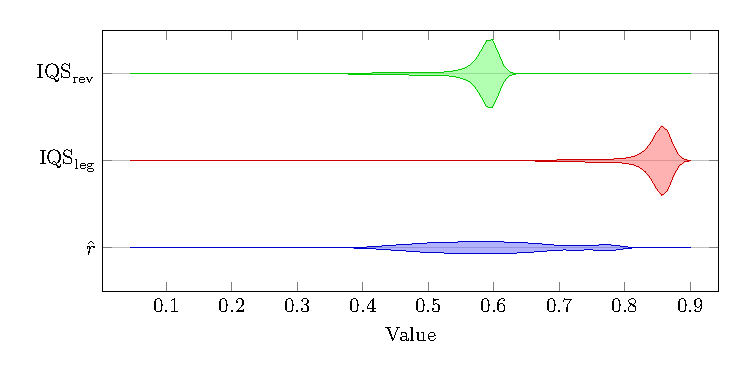
\includegraphics[width=1\linewidth]{figures/violin.pdf}
    \caption{Violin plot comparing the distributional shapes of $\iqsleg$, $\iqsrev$, and $s$. The proposed score exhibits a broader, flatter density, reflecting enhanced discriminability across the score domain.}
    \label{fig:violin}
\end{figure}

To spatially validate the framework, we consider a single evaluation frame representing the period of December 2022. Fig.~\ref{fig:mps} shows the comparative geographic mapping for each metric across Brazilian municipalities. The map visualization corroborates the distributional patterns observed in the violin analysis. While the \gls{gnn} score exhibits continuous performance transitions that clearly highlight distinct geographic regions, the traditional indicators cluster the vast majority of municipalities into the highest or a narrow middle tier.

The geographic contrast is particularly evident when comparing macro-regions. In the $\iqsleg$ map, municipalities in the South and Southeast regions---which concentrate the country's telecommunications infrastructure---appear visually indistinguishable from well-connected cities in the North and Northeast, as both are mapped to the same narrow high-score band. This saturation masks known infrastructure disparities between these regions. The $\iqsrev$ map, despite its performance-weighted scheme, exhibits a similar lack of regional differentiation, with most of the territory rendered in a uniform mid-tone.

In contrast, the proposed model's score map reveals a clear North--South gradient consistent with known patterns of infrastructure deployment and population density. Municipalities in the South, Southeast, and parts of the Center-West display higher scores, forming distinguishable clusters, while the North and parts of the Northeast exhibit lower scores that reflect documented challenges in coverage and connectivity. Importantly, even within macro-regions the model captures intra-regional heterogeneity: isolated high-performing municipalities (typically state capitals or large urban centers) are clearly visible against their surrounding rural areas, a distinction that the baselines' compressed ranges cannot render.

\begin{figure*}[t]
    \centering
    \begin{subfigure}[b]{0.32\textwidth}
        \centering
        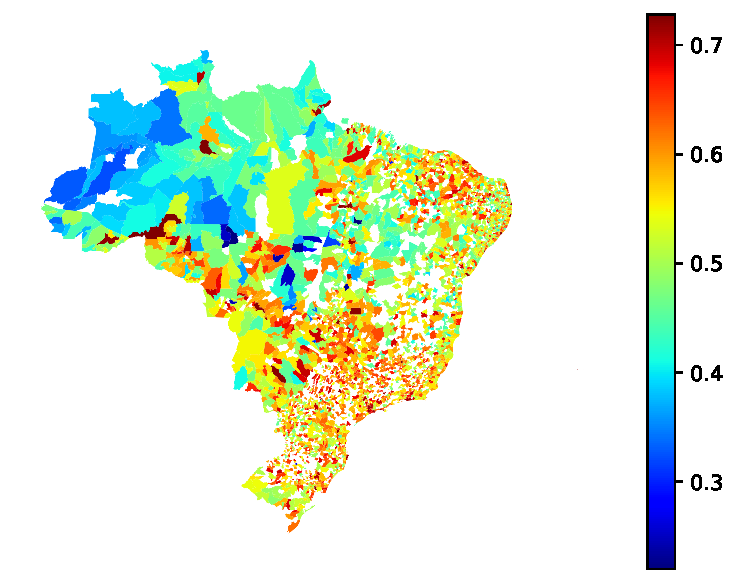
\includegraphics[width=\textwidth]{figures/map_score.pdf}
        \caption{Manifold Ranker $s$}
        \label{fig:map_s}
    \end{subfigure}
    \hfill
    \begin{subfigure}[b]{0.32\textwidth}
        \centering
        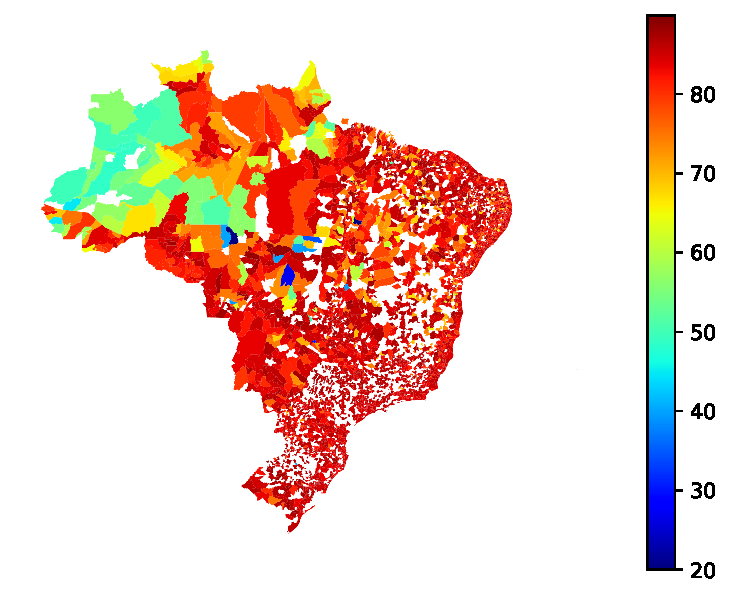
\includegraphics[width=\textwidth]{figures/map_iqs_old.pdf}
        \caption{$\iqsleg$}
        \label{fig:map_iqs_leg}
    \end{subfigure}
    \hfill
    \begin{subfigure}[b]{0.32\textwidth}
        \centering
        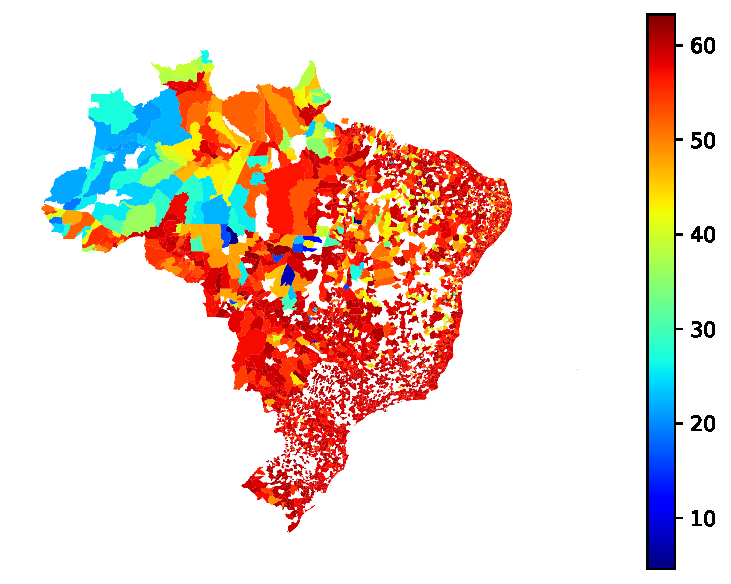
\includegraphics[width=\textwidth]{figures/map_iqs_new.pdf}
        \caption{$\iqsrev$}
        \label{fig:map_iqs_ev}
    \end{subfigure}
    
    \caption{Geographic distribution of scores for $\iqsleg$, $\iqsrev$, and $s$ for December 2022. The model score reveals spatial heterogeneity masked by the baselines' narrow ranges.}
    \label{fig:mps}
\end{figure*}

\section{Conclusions} \label{sec:conclusions}

In this paper, we introduced Manifold Ranker, a \gls{gnn}-based self-supervised framework designed to resolve ranking limitations in telecommunications quality assessment. While current regulatory composites---the legacy and revised \gls{iqs}---suffer from severe score clustering that limits spatial and technical discrimination, our proposed model effectively leverages manifold structure through graph-based message passing and a multi-objective loss function.

By combining pairwise ranking, feature reconstruction, geometric smoothness, and a directional compass penalty, the model's optimization covers distinct perspectives that complement each other, yielding a more balanced solution than unidimensional scalar optimization alone. The quantitative analysis confirms this: the proposed score achieves an interquartile range of $0.137$, representing a nearly $5\times$ expansion compared to both baselines (IQR $= 0.028$), and a standard deviation $1.8\times$ larger than the legacy \gls{iqs}. This expanded range directly translates into improved discriminability, as demonstrated by the distributional and geographic analyses.

For future work, we plan to benchmark the proposed approach against established Learning to Rank baselines in the literature. Furthermore, there is potential in expanding this analysis to other socioeconomic domains. Finally, exploring alternative positional encoding methods, such as Spectral Embedding for non-linear manifold coordinates, and testing other activation functions to assess structural stability, remain planned efforts for subsequent research.

% \section*{Acknowledgments}

% \bibliographystyle{IEEEtran}
% \bibliography{references}

\end{document}
